\section{Enhancing transcriptomic reference}

The enhanced transcriptomic reference allows to include those reads into downstream analysis that otherwise would be discarded.
To achieve this, we have combine data from several different transcriptomic annotations,
and additionally included in the annotation intergenic regions that contained relativelly high number of reads.

\input{"data/downstream/summaries/count_summaries/count_summary.tex"}

\subsection{Exploring unassigned reads}
Unassigned reads could come from several sources:
sequencing artefacts, genes that are not included into transcriptomic reference used, or genes that are not annotated yet.
To check, we have looked at intersections of those unassigned reads and more comprehensive annotations.
As we can see, that there are plenty of genes from more comprehensive annotations which intersect with unassigned genes,
and number of those intersecting genes correlates with sequencing depth.

\input{"data/downstream/summaries/gene_summaries/intersecting_gene_summary.tex"}

\input{"data/downstream/summaries/captured_gene_summaries/captured_gene_types_summary.tex"}

\subsection{Intergenic regions}

Observed intergenic regions can be either artefacts or be biologically meaningfull.
To check this, I have tried to cluster cells based only on the newly defined intergenic regions (see figure \ref{fig:umapComparisonIntergenic}).
While for PBMC\_indrops sample it looks as noise, for the 10x indrops samples it provides quite good clustering,
meaning that at least some of those captured intergenic regions are not sequencing artefacts.

\begin{figure}[htbp]
    \centering
    \begin{subfigure}{0.45\textwidth}
        \centering
        \includegraphics[width=\textwidth]{images/umaps/intergenic_10x_indrops.png}
        \caption{Indrops PBMC}
    \end{subfigure}
    \hfill
    \begin{subfigure}{0.45\textwidth}
        \centering
        \includegraphics[width=\textwidth]{images/umaps/intergenic_10x_pbmc10x1.png}
        \caption{10x PBMC 1}
    \end{subfigure}
    \vspace{0.5em}
    \begin{subfigure}{0.45\textwidth}
        \centering
        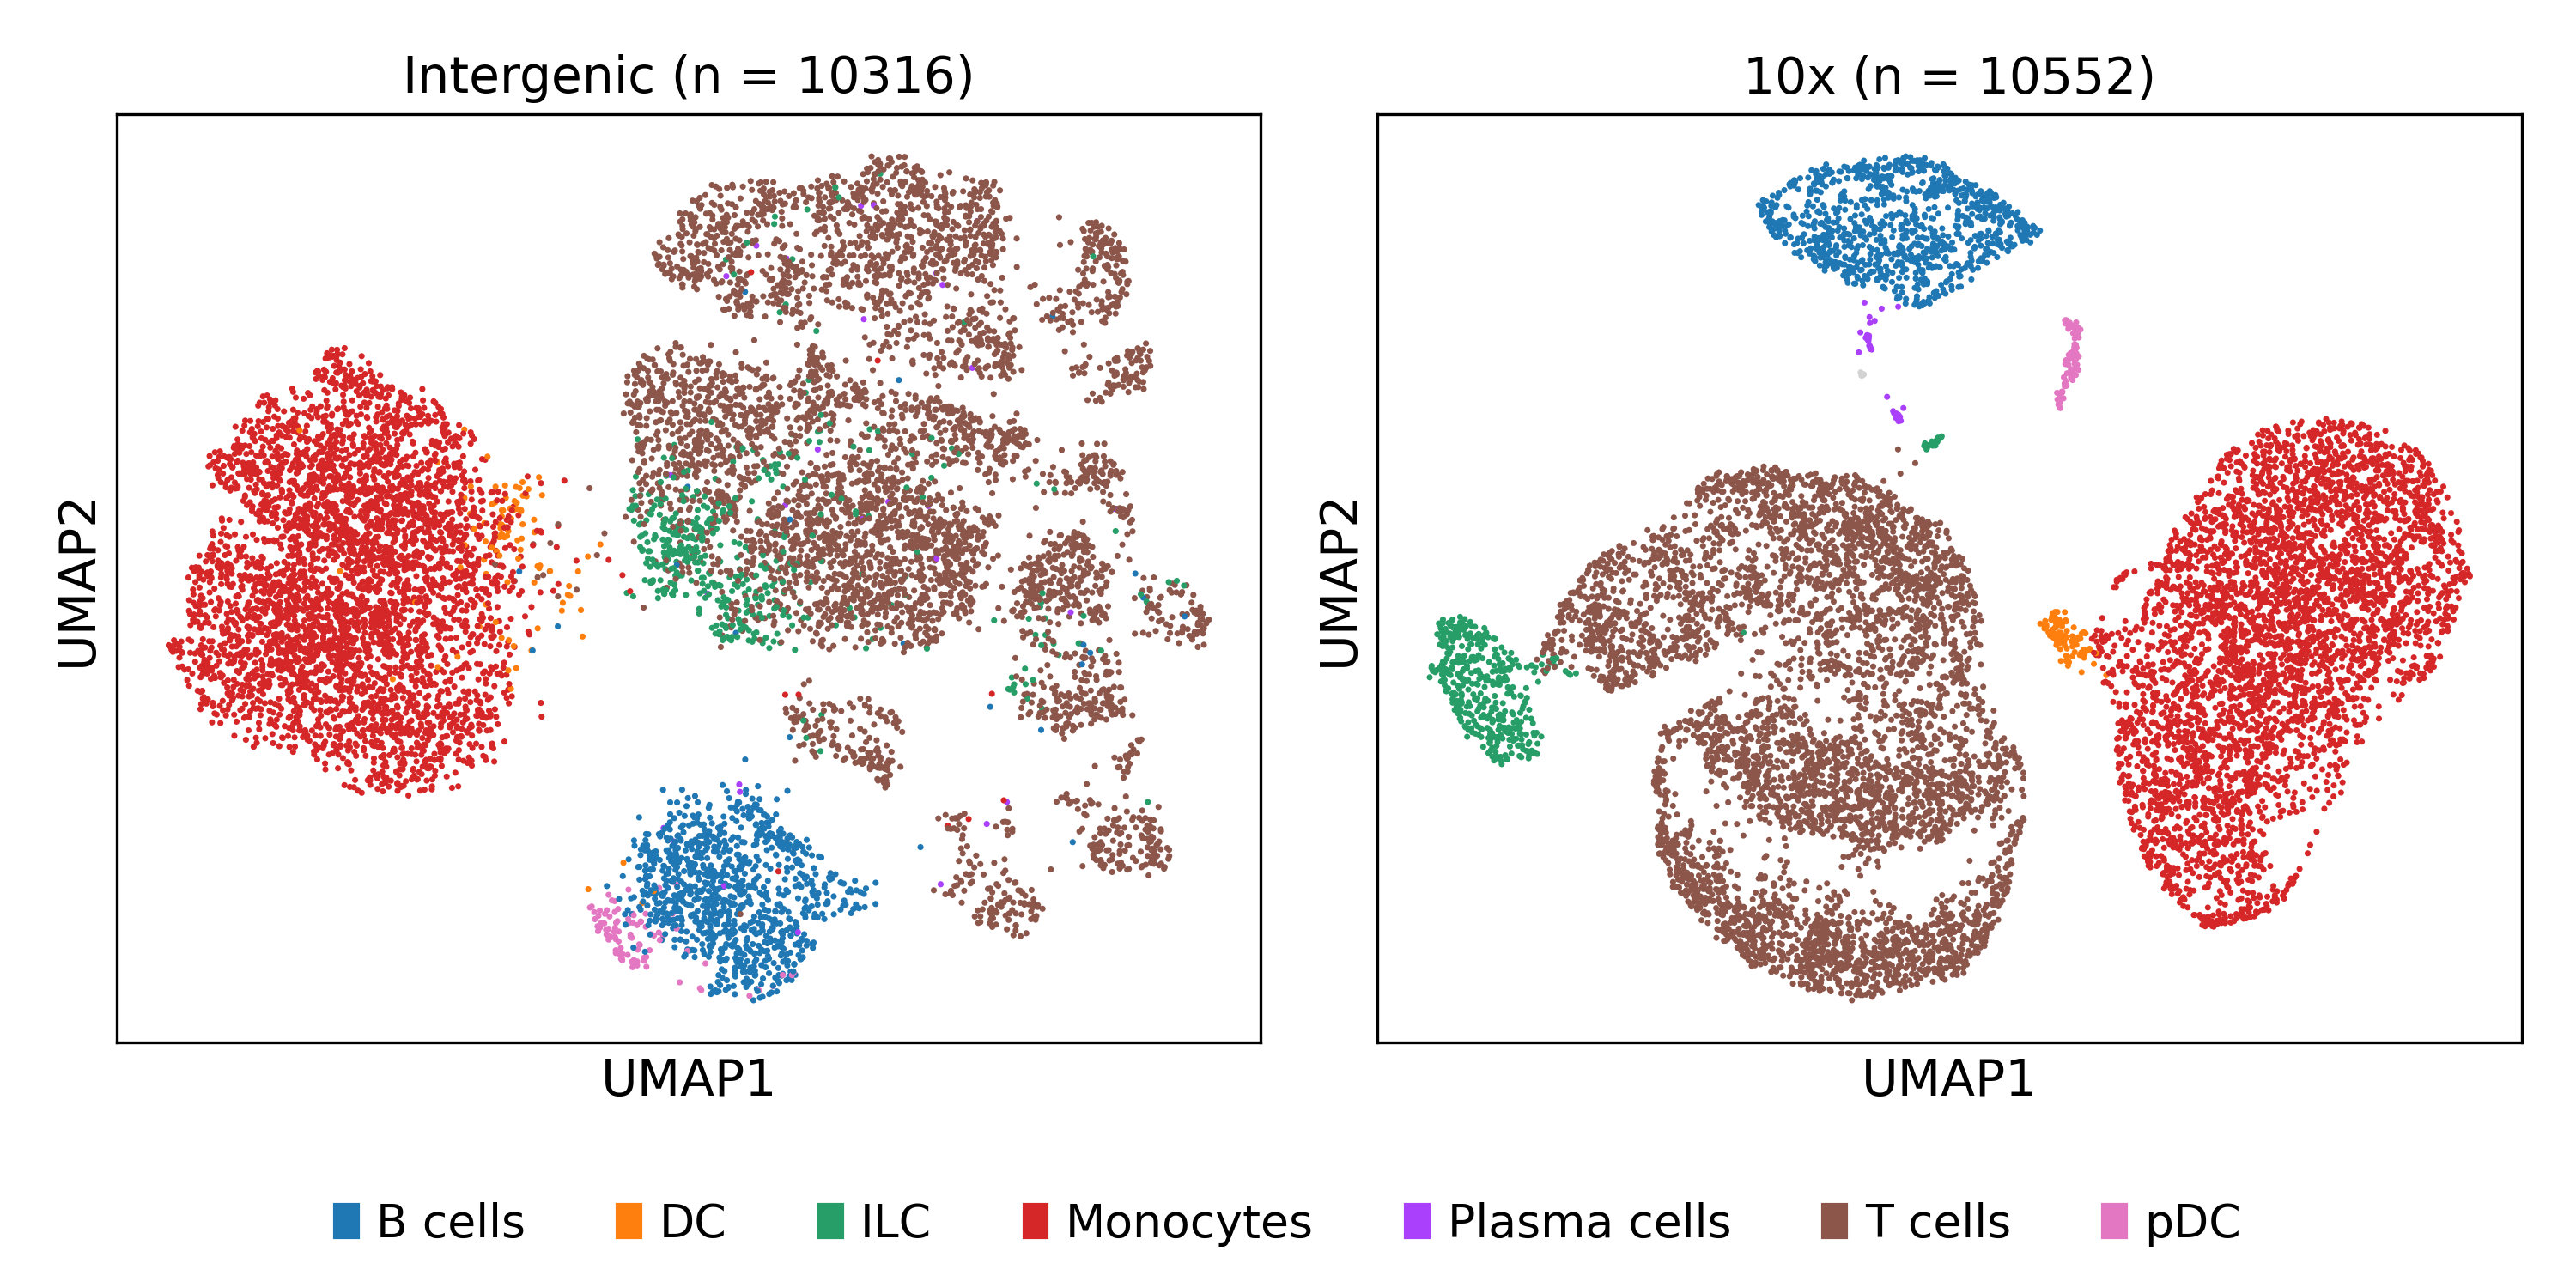
\includegraphics[width=\textwidth]{images/umaps/intergenic_10x_pbmc10x2.png}
        \caption{10x PBMC 2}
    \end{subfigure}
    \hfill
    \begin{subfigure}{0.45\textwidth}
        \centering
        \includegraphics[width=\textwidth]{images/umaps/intergenic_10x_brain.png}
        \caption{10x Brain}
    \end{subfigure}
    \caption{Comparison of clustering using only intergenic regions versus standard (10x) reference.
    'Intergenic' plots are colored according to the '10x' coloring.}
    \label{fig:umapComparisonIntergenic}
\end{figure}

\subsection{Enhanced Reference}

Using enhanced reference allowed us to have more captured genes in the data,
however, no significant change in clustering can be seen.

\subsection{Captured genes}


